%%%%%%%%%%%%%%%%%%%%%%%%%%%%%%%%%%%%%%%%%%%%%%%%%%%%%%%%%%%%%%%
%                                                             %
%                     SNU_sample.tex v1.1                     % 
%                                - fixed by SH Park (SNU ASL) %
%                                - GitHub: WhenTheyCry96      % 
%                                                             %
%%%%%%%%%%%%%%%%%%%%%%%%%%%%%%%%%%%%%%%%%%%%%%%%%%%%%%%%%%%%%%%

% 논문작성을 위해서 한글패키지가 설치되어 있어야 합니다.
% MikTeX 을 사용할 것을 권장하며, MikTeX의 설치 및 한글 패키지와 관련된 사항은
% KTUG 한글 TeX 사용자 그룹 http://www.ktug.or.kr을 참조하시길 바랍니다.
%
% 본 tex file의 여백은 B5(JIS)에 맞춰져 있습니다.
% 컴파일을 완료하고 ps file을 생성한뒤, command prompt에서
% dvips -T 182mm,257mm -o Snu_sample.ps Snu_sample.dvi명령어를
% 사용하여 .ps file을 생성하면 됩니다.
%
% ps file을 pdf로 변환한 뒤에, 인쇄시 B5(JIS)에 맞춰서 출력하고,
% 옵션중 페이지 비율을 없음으로 해야 원하는 여백 그대로 출력됩니다.
%

% SNU_template.cls file을 사용합니다.
% 박사의 경우 \documentclass[doctor]{SNU_template} (default)
% 석사의 경우 \documentclass[master]{SNU_template} 로 변경하면 됩니다.
% SNU_template.cls file명이 바뀔경우에는 {SNU_template} 대신에 {바뀐 file명}을 넣으면 됩니다.
% 주어진 .cls file의 내용을 변경하는 것은 규격에 어긋난 결과를 낼 수 있습니다.
%
% 주어진 .cls file은 서울대학교 논문 규격에 맞춰서 작성되어 있으며,
% MS Word 양식과 동일한 output을 내도록 작성되어 있으므로
% 특별한 설명이 없는 부분은 Word양식의 guideline을 참조하시면 됩니다.

\documentclass[doctor]{snuee}
\usepackage{filecontents}
\usepackage{graphicx}
\usepackage{amsmath}
\usepackage{lipsum}
\usepackage{cite}
% rotating은 테이블을 한 페이지에 크게 옆으로 생성할 수 있게 하는 패키지입니다. 필요없으시면 주석처리하시면 됩니다.
\usepackage{rotating}
% hyperref는 레퍼런스를 누르면 이동하는 패키지입니다. 필요없으시면 주석처리하시면 됩니다.
\usepackage[colorlinks=true, linkcolor=black, citecolor=black]{hyperref} 
% appendix는 appendix 이쁘게 나오게하는 패키지입니다. 필요없으시면 주석처리하시면 됩니다.
\usepackage[titletoc]{appendix}

% reference bibtex format용도입니다. Ref.bib 의 첫번째 커맨드를 보시면 저자 수에 따른 et al 사용 등 조절 가능.
\makeatletter
\def\bstctlcite{\@ifnextchar[{\@bstctlcite}{\@bstctlcite[@auxout]}}
\def\@bstctlcite[#1]#2{\@bsphack
  \@for\@citeb:=#2\do{%
    \edef\@citeb{\expandafter\@firstofone\@citeb}%
    \if@filesw\immediate\write\csname #1\endcsname{\string\citation{\@citeb}}\fi}%
  \@esphack}
\makeatother 

% 피규어들의 폴더 경로를 알아서 figure 폴더로 잡는 줄입니다. 필요없으시면 주석처리하시면 됩니다.
\graphicspath{{figure/}}
% 편하게 이미지를 넣으시고 싶으실 경우, 확장자를 미리 정의하실 수 있습니다.
% \DeclareGraphicsExtensions{.png}

% 논문 작성을 위한 사전 준비과정
% 논문제목 (국문, 영문), 저자, 제출일, 심사일, 졸업일의 정보를 넣습니다.

% 논문제목을 넣습니다.
% 필히 한글제목과 영문제목 모두 넣어야 합니다.
\title[korean]{서울대학교 박사학위 제목}                % FIXME
\title[english]{Title of SNU PhD Dissertation Thesis} % FIXME

% 저자 정보를 넣습니다.
% 국문성명, 영문성명 모두 넣어야 하며, 특히 국문성명의 경우는 글자사이에 space가 있는 것과 없는 것
% 두 가지 모두를 집어넣어줘야 합니다.
\author[korean]{홍 길 동}      % FIXME
\author[english]{Hong Gildong} % FIXME
\author[nospace]{홍길동}       % FIXME

% 지도교수님의 성함을 국문으로 넣습니다.
\adviser{김철수} % FIXME

% 논문 제출일, 논문 심사일을 한글로 넣습니다.
\submissiondeadline{2022년 8월} \examinationdate{2022년 6월}  % FIXME

% 졸업일을 영문식, 한글식 두 가지 방법 모두 넣습니다.
\gradyear[english]{AUGUST 2022} \gradyear[korean]{2022년 8월} % FIXME

%

% 문서의 시작
%
% 위의 정보들을 빠짐없이 채워넣고 document를 시작하면
% 외표지, 내표지(외표지와 동일), 인준지가 자동으로 생성됩니다.

\begin{document}
\bstctlcite{IEEEexample:BSTcontrol}
\renewcommand{\baselinestretch}{1.5}    % 본문의 줄간격 조정, 고치거나 삭제하지 마십시오.
\selectfont                             

% abstract(영문)의 작성
% begin과 end 사이에 abstract의 내용을 채워넣습니다.
\begin{abstract}
	\par %abstract 첫 문장 들여쓰기, 고치거나 삭제하지 마십시오.
%% 다시 쓰기, 여러 문단으로 구성해도 됨. 2~7페이지 분량으로 쓰면 됨. 현재는 1페이지
	README (FIXME)
	This tex file gives you guidelines for preparing thesis of School of Electrical Engineering.
	This document can be used as a template for the thesis.
	You can easily make your thesis document using this template. You can freely put your chapters,
	sections in this tex file.
	Do not change SNU\_template.cls file and do not remove specified
	command lines in this sample file.
	Title and other information in abstract like name and affiliation can be
	omitted. Keywords and student number should be located at bottom of
	page. We hope this document be helpful to writing a thesis. Paper
	size is B5(JIS:182mmX257mm), all English character font type is
	Times New Roman, Korean character font type is MyoungJo(명조체).
	Line spacing, paper margin and other additional informations are
	indicated in Description.doc in MS Word template.

	The caption of the figure should be located below the figure and end with `.'
	If the caption of the figure is longer than one lines, you should align it left.(This is default)
	The caption of the table should be located above the table. Be careful that caption should not end with `.'
	% abstract page 하단에 keyword와 학번을 넣습니다.
	\vfill
	\begin{minipage}[t][20mm][b]{\textwidth}
		{\bfseries Keywords}: keyword1, keyword2, keyword3, keyword4, lessthan, 6keywords \\ % FIXME
		{\bfseries Student Number}: 2000-00000\\                        % FIXME
	\end{minipage}
	
\end{abstract}

\changepage{5mm}{}{}{}{}{}{}{}{-5mm}    %%페이지 여백 재설정. 절대 고치거나 삭제하지 마십시오.
\makelists   %목차를 자동생성합니다.

% 본문의 시작
% chapter, section의 추가,변경등 모두를 자유롭게 할 수 있습니다.
% 그림, 표의 추가 형식은 MS Word의 형식과 동일합니다. (MS Word Description file 참조)
% Nomenclature 컴파일 하는 방법
% 아래 명령어 실행 (본 main.tex의 경우에는, 파일명에 main로 치환해서 돌리면 됩니다.)
% makeindex -s nomencl.ist -t "파일명.nlg" -o "파일명.nls" "파일명.nlo" 
%=========================================================================================================================================================
%=========================================================================================================================================================

% FIXME
\nomenclature{\(c\)}{Speed of light in a vacuum}
\nomenclature{\(h\)}{Planck constant}
\nomenclature{\(+a\)}{Operator}
\nomenclature{\(2a\)}{Number}
\nomenclature{\(:a\)}{Punctuation symbol}
\nomenclature{\(Aa\)}{Uppercase letter}
\nomenclature{\(aa\)}{Lowercase letter}
\nomenclature{\(\hat{H}\)}{Hamiltonian}
\nomenclature{\(\hat{a}^{\dag}_i\)}{Creation operator}
\nomenclature{\(\alpha\)}{Greek character}

%=========================================================================================================================================================
%=========================================================================================================================================================


\chapter{INTRODUCTION}
\lipsum[1-4]~\cite{anderson1964hard}

\section{Intro:section I}
\lipsum[1-4]~\cite{anderson1964hard}

\begin{figure}[!t]
	{
	\begin{center}
		\begin{tabular}{c}
			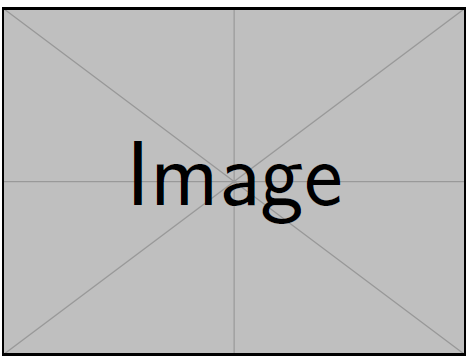
\includegraphics[width=0.9\linewidth]{dummy.png}
		\end{tabular}
	\end{center}
	}
	\caption[dummy image FIXME1]{Figure option of $!\text{t}$.}
\label{dummy_img1}
\end{figure}

\subsection{Intro:section I-1}
\lipsum[1-4]~\cite{anderson1964hard}

\begin{figure}[!b]
	{
	\begin{center}
		\begin{tabular}{c}
			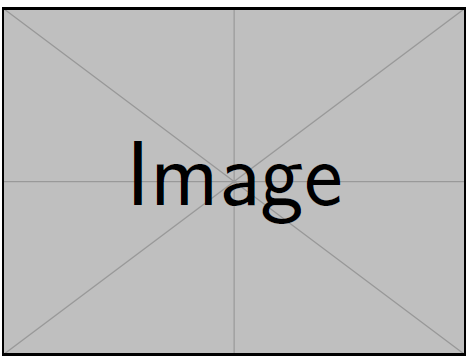
\includegraphics[width=0.9\linewidth]{dummy.png}
		\end{tabular}
	\end{center}
	}
	\caption[dummy image FIXME2 with long long long long long long long title]{Figure option of $!\text{b}$.}
\label{dummy_img2}
\end{figure}

\section{Intro:section II}
\lipsum[1-4]~\cite{anderson1964hard}

\begin{table}[htbp]
	\renewcommand{\arraystretch}{1.6}
	\setlength{\tabcolsep}{10pt}
	\caption{Table caption goes up FIXME}
	\label{tbl2_1}
	\centering
	\begin{tabular}{l l l l l l c}
	\hline\hline
	Material & $T_c$ & $B_c$& $\xi$ & $\lambda_L$ & $\kappa$ & Type \\
	\hfill & [K] & [T] & [nm] & [nm] & \hfill & \hfill \\
	\hline
	FIXME & 1 & 2 & 3 & 4 & 5 & FIXME \\
	\hline\hline
	\end{tabular}
\end{table}

\subsection{Intro:section II-1}
\lipsum[1-4]~\cite{anderson1964hard}

\begin{sidewaystable}[htbp]
	\renewcommand{\arraystretch}{1.2}
	\setlength{\tabcolsep}{5pt}
	\centering
	\footnotesize
	\begin{tabular}{l c c c c c c c c c c c c c c c c c c c}
	\hline
	Parameter (FIXME) & P1 & P2 & P3 & P4 & P5 & P6 & P7 & P8 & P9 & P10\\
	\hline
	\multicolumn{11}{l}{\textbf{Conductor configuration}}\\
	$P_{FIXME}$\hfill[A]& FIXME & FIXME & FIXME & FIXME & FIXME & FIXME & FIXME & FIXME & FIXME & FIXME\\
	\hline
	\end{tabular}
	\caption{Key parameters of FIXME sideway table.}
	\label{tbl2-2}
\end{sidewaystable} % FIXME (introduction)
\chapter{BACKGROUND}
\lipsum[1-4]~\cite{anderson1964hard}

\section{Back:section I}
\lipsum[1-4]~\cite{anderson1964hard}
\begin{table}[htbp]
	\renewcommand{\arraystretch}{1.6}
	\setlength{\tabcolsep}{10pt}
	\caption{Table caption goes up FIXME2}
	\label{tbl3_1}
	\centering
	\begin{tabular}{l l l l l l c}
	\hline\hline
	Material & $T_c$ & $B_c$& $\xi$ & $\lambda_L$ & $\kappa$ & Type \\
	\hfill & [K] & [T] & [nm] & [nm] & \hfill & \hfill \\
	\hline
	FIXME & 1 & 2 & 3 & 4 & 5 & FIXME \\
	\hline\hline
	\end{tabular}
\end{table}

\subsection{Back:section I-1}
\lipsum[1-4]~\cite{anderson1964hard}

\section{Back:section II}
\lipsum[1-4]~\cite{anderson1964hard}

\subsection{Back:section II-1}
\lipsum[1-4]~\cite{anderson1964hard} % FIXME (background)
\chapter{DISCUSSION}
\lipsum[1-4]~\cite{anderson1964hard}

\section{Discussion:section I}
\lipsum[1-4]~\cite{anderson1964hard}

\subsection{Discussion:section I-1}
\lipsum[1-4]~\cite{anderson1964hard}
 % FIXME (discussion)
\chapter{CONCLUSION}
\lipsum[1-4]~\cite{anderson1964hard} % FIXME (conclusion)

% appendix 필요없으면 아래의 % start appendices FIXME
%%%%%%%%%%%%%%%%%%%%DO NOT MODIFY THIS PART%%%%%%%%%%%%%%%%%%%%%%%%%%%
\appendix
% \clearpage % or \cleardoublepage
\newpage
\makeatletter
\makeatother
\begin{appendices}
\chapter*{Appendix}
\addcontentsline{toc}{chapter}{}
% 밑의 sectioning이 ToC에서 보이고 싶은 느낌따라서,
% Appendix A.1 <-- \Alph
% Appendix 1.1 <-- \arabic 
% 중 선택하세요.
\renewcommand{\thesection}{\Alph{section}}
\renewcommand\thetable{\thesection.\arabic{table}}  
\renewcommand\thefigure{\thesection.\arabic{figure}}  
%%%%%%%%%%%%%%%%%%%%%%%%%%%%%%%%%%%%%%%%%%%%%%%%%%%%%%%%%%%%%%%%%%%%%%

\section{First Appendix}
\subsection{FIXME Appendix1}
\lipsum[1-2]~\cite{anderson1964hard}
\begin{figure}[!t]
	{
	\begin{center}
		\begin{tabular}{c}
			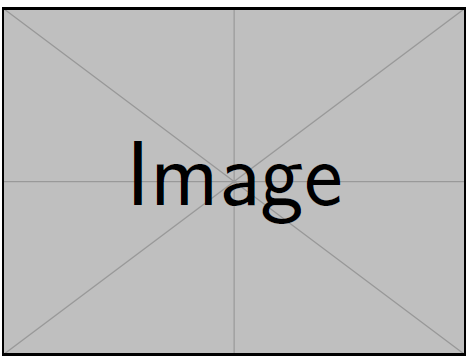
\includegraphics[width=0.9\linewidth]{dummy.png}
		\end{tabular}
	\end{center}
	}
	\caption[dummy image FIXME A1]{Figure option of $!\text{t}$.}
\label{dummy_imgA1}
\end{figure}
\subsection{FIXME Appendix2}
\begin{table}[htbp]
	\renewcommand{\arraystretch}{1.6}
	\setlength{\tabcolsep}{10pt}
	\caption{Table caption goes up FIXME A1}
	\label{tbl3_1}
	\centering
	\begin{tabular}{l l l l l l c}
	\hline\hline
	Material & $T_c$ & $B_c$& $\xi$ & $\lambda_L$ & $\kappa$ & Type \\
	\hfill & [K] & [T] & [nm] & [nm] & \hfill & \hfill \\
	\hline
	FIXME & 1 & 2 & 3 & 4 & 5 & FIXME \\
	\hline\hline
	\end{tabular}
\end{table}
\lipsum[1-2]~\cite{anderson1964hard}

\end{appendices}
% end appendices 줄 주석처리 하세요.
% start appendices FIXME
%%%%%%%%%%%%%%%%%%%%DO NOT MODIFY THIS PART%%%%%%%%%%%%%%%%%%%%%%%%%%%
\appendix
% \clearpage % or \cleardoublepage
\newpage
\makeatletter
\makeatother
\begin{appendices}
\chapter*{Appendix}
\addcontentsline{toc}{chapter}{}
% 밑의 sectioning이 ToC에서 보이고 싶은 느낌따라서,
% Appendix A.1 <-- \Alph
% Appendix 1.1 <-- \arabic 
% 중 선택하세요.
\renewcommand{\thesection}{\Alph{section}}
\renewcommand\thetable{\thesection.\arabic{table}}  
\renewcommand\thefigure{\thesection.\arabic{figure}}  
%%%%%%%%%%%%%%%%%%%%%%%%%%%%%%%%%%%%%%%%%%%%%%%%%%%%%%%%%%%%%%%%%%%%%%

\section{First Appendix}
\subsection{FIXME Appendix1}
\lipsum[1-2]~\cite{anderson1964hard}
\begin{figure}[!t]
	{
	\begin{center}
		\begin{tabular}{c}
			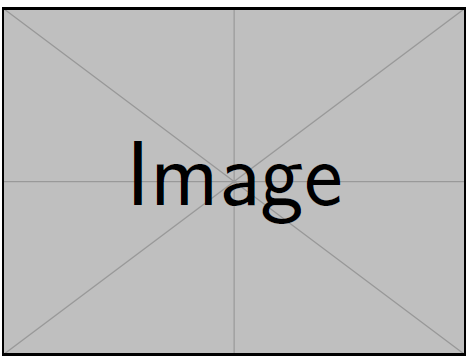
\includegraphics[width=0.9\linewidth]{dummy.png}
		\end{tabular}
	\end{center}
	}
	\caption[dummy image FIXME A1]{Figure option of $!\text{t}$.}
\label{dummy_imgA1}
\end{figure}
\subsection{FIXME Appendix2}
\begin{table}[htbp]
	\renewcommand{\arraystretch}{1.6}
	\setlength{\tabcolsep}{10pt}
	\caption{Table caption goes up FIXME A1}
	\label{tbl3_1}
	\centering
	\begin{tabular}{l l l l l l c}
	\hline\hline
	Material & $T_c$ & $B_c$& $\xi$ & $\lambda_L$ & $\kappa$ & Type \\
	\hfill & [K] & [T] & [nm] & [nm] & \hfill & \hfill \\
	\hline
	FIXME & 1 & 2 & 3 & 4 & 5 & FIXME \\
	\hline\hline
	\end{tabular}
\end{table}
\lipsum[1-2]~\cite{anderson1964hard}

\end{appendices}
% end appendices % FIXME
%=========================================================================================================================================================
%=========================================================================================================================================================

% 참고문헌을 넣습니다.
% 샘플의 형식과 같은 차례대로 써줍니다.


\bibliographystyle{IEEEtran} % FIXME
\bibliography{Ref}           % FIXME

%\begin{thebibliography}{00}

	% 영문저널의 경우
%	\bibitem{ref1} B. Jeon and J. Jeong, ``Blocking artifacts
%	reduction in image compression with block boundary discontiunity
%	criterion,'' {\em IEEE Transactions on Circuits and Systems for
%		Video Tech.}, vol. 8, no.3, pp. 345-357, June 1998.
	
	% 영문학술대회의 경우
%	\bibitem{ref2} W. G. Jeon and Y. S. Cho, ``An equalization
%	technique for OFDM and MC-CDMA in a multipath fading channels,''
%	in {\em Proceedings of IEEE Conference on Acoustics, Speech and
%		Signal Processing}, Munich, Germany, May 1997. pp. 2529-2532.
	
	% 국내저널의 경우
%	\bibitem{ref3} 김남훈, 정영철, ``평탄한 통과대역 특성을 갖는
%	새로운 구조의 광도 파로열 격자 라우터,'' {\em 전자공학회논문지},
%	제35권 D편, 제3호, 56-62쪽, 1998년 3월.
	
	% 국내학술대회의 경우
%	\bibitem{ref4} 윤남국, 김수종, ``무선 센서 네트워크에서의 에너지
%	효율적인 그라디언트 기반 라우팅 기법,'' {\em 한국정보과학회
%		2006년 추계학술대회}, 제12권, 제2호, 2006년 10월. pp.
%	1372-1374.
	
	% 단행본의 경우
%	\bibitem{ref5} C. Mead and L. Conway, {\em Introduction to VLSI
%		Systems}, Addison-Wesley, Boston, 1994.
	
	% URL
%	\bibitem{ref6} The SolarMESH Network,
%	http://owl.mcmater.ca/solarmesh
	
	% Technical Report의 경우
%	\bibitem{ref7} K. E. Elliott and C. M. Greene, ``A local adaptive
%	protocol,'' Argonne National Laboratory, Argonne, France,
%	Technical Report 916-1010-BB, 1997.
	
	% 학위논문의 경우
%	\bibitem{ref8} T. Kim, ``Scheduling and Allocation Problems in
%	High-level Synthesis,'' Ph. D. Dissertation, ECE Department,
%	Univ. of Illinois at U-C, 1993.
	
	% 특허의 경우
%	\bibitem{ref9} Sunghyun Choi, ``Wireless MAC protocol based on a
%	hybrid combination of slot allocation, token passing, and
%	polling for isochronous traffic,'' U.S. Patent No. 6,795,418,
%	September 21, 2004.
	
	% 표준
%	\bibitem{ref10} IEEE Std. 802.11-1999, Part 11: Wireless LAN
%	Medium Access Control (MAC) and Physical Layer (PHY)
%	specifications, Reference number ISO/IEC 8802-11:1999(E), IEEE
%	Std. 802.11, 1999 edition, 1999.
	
%\end{thebibliography}

%=========================================================================================================================================================
%=========================================================================================================================================================

% 본문의 종료
% 국문 초록과 감사의 글(선택)을 넣습니다.
% begin{summary}와 end{summary}의 사이에 국문초록을 집어넣습니다.
% 감사의글은 \acknowledgement{}의 대괄호 안에 내용을 넣습니다.
%
\begin{summary}
	\par    %첫 줄 들여쓰기를 위한 단락구분.삭제하지 마십시오.
	국문 초록 FIXME 꼭 고쳐주십시오. 
	
	\lipsum[1-3]
	\lipsum[1-3]
	\vfill
	\begin{minipage}[t][20mm][b]{\textwidth}
		{\bfseries 주요어}: 서울대학교 논문양식, TeX\\
		{\bfseries 학번}: 2000-00000\\
	\end{minipage}
\end{summary}
\changepage {-15mm}{}{}{}{}{}{}{}{15mm} % 수정된 초록과 감사의 글을 위한 여백 재설정!
% \changepage {15mm}{}{}{}{}{-30mm}{}{}{15mm} %초록과 감사의 글을 위한 여백 재설정, 고치거나 삭제하지 마십시오. (원래 포맷)

%=========================================================================================================================================================
%=========================================================================================================================================================

\acknowledgement{
	\par
	Put your acknowledgement here.(optional)} %감사의 글을 작성하지 않을경우 삭제가능
\end{document}
